\documentclass[runningheads]{llncs}

\usepackage[T1]{fontenc}
\usepackage[utf8]{inputenc}
\usepackage{amsmath}
\usepackage{graphicx}
\usepackage{url}
\usepackage{array}
\usepackage{booktabs}
\usepackage{multirow}

\begin{document}

\title{Runtime-Side Security Profile Generation for OCI Containers}
\titlerunning{Runtime-Side Security Profile Generation}

\author{Ivan Platonov\inst{1} \and Andrey Sadovykh\inst{2} \and Kirill Saltanov\inst{3}}
\authorrunning{I. Platonov, A. Sadovykh, K. Saltanov}
\institute{Innopolis University, Innopolis, Russia\\
\email{i.platonov@innopolis.university}
\and
Softeam, Paris, France\\
\email{andrey.sadovykh@softeam.fr}
\and
Innopolis University, Innopolis, Russia\\
\email{kirill.saltanov@innopolis.university}}

\maketitle

\begin{abstract}
With growing adoption of OCI containers and increasingly automated offensive tooling, protecting containerised workloads without a dedicated DevSecOps stack remains difficult. Sandboxed runtimes such as gVisor reduce kernel exposure but impose substantial steady-state overhead. Manual seccomp, AppArmor, and capability authoring requires kernel expertise that most teams cannot sustain. Cluster-side recorders such as the Kubernetes Security Profiles Operator and Inspektor Gadget assume orchestration infrastructure, persistent storage, and profile-pinning workflows.

This paper presents a security-oriented fork of \texttt{runc} (\texttt{dpttk/runc}, version~1.4.0-rc.1) in which profile generation is performed by the runtime itself. On a designated scanning invocation, the runtime relaxes confinement in memory, traces kernel interactions through \texttt{oci-seccomp-bpf-hook}, cgroup-scoped \texttt{capable-bpfcc}, and AppArmor complain mode, and writes a workload-specific seccomp allow-list, AppArmor profile, and minimised capability set back into the OCI bundle. Subsequent runs enforce these artefacts as ordinary OCI inputs; tracing logic ships as hidden sub-commands of the runtime binary, so the bundle gains data artefacts only.

We evaluate the runtime on three axes. \textbf{Profile quality and containment} are measured on the \texttt{runc-hardened-test} laboratory: a single \texttt{--security-scan} pass produces deny-by-default policies, and scan-then-enforce blocks command-injection payloads that succeed under stock \texttt{runc} while preserving legitimate application traffic. \textbf{Enforcement overhead} is measured on four container workloads (sysbench CPU/memory, loopback iperf3, redis-benchmark) with 50 repetitions after warm-up: median throughput loss of the enforced configuration relative to the same binary without profiles is below 1\% on CPU, memory, and network workloads and about 5.5\% on Redis SET/GET. \textbf{Sandbox positioning} on the same host shows gVisor 2.6--73\% below Docker-default throughput depending on workload. Additional escape-class evaluations beyond the Flask laboratory are planned and left as explicit placeholders in Section~\ref{sec:eval-security-planned}.

\keywords{OCI runtime \and runc \and seccomp \and AppArmor \and Linux capabilities \and eBPF.}
\end{abstract}

\section{Introduction}

Containers are now a standard deployment unit for cloud applications, but their isolation boundary remains fundamentally different from a virtual machine boundary. A container usually shares the host kernel with other workloads on the node, so kernel-facing attack surface matters directly to tenant isolation and host integrity~\cite{wang2022,flauzac2020}. The Open Container Initiative (OCI) standardises the runtime contract, and \texttt{runc} remains the reference implementation used under many higher-level stacks. Its strength is compatibility and low overhead; its weakness is that strong confinement depends on policies supplied by the operator.

Linux already exposes the mechanisms required for a narrower boundary: seccomp filters syscalls, AppArmor restricts path-based filesystem access, and Linux capabilities split privileged root operations into smaller units. The problem is not the absence of mechanisms, but the cost of producing profiles that are strict enough to be useful and still broad enough not to break the workload.

This paper asks whether the runtime itself can reduce that cost. The proposed system is a fork of \texttt{runc} with a scanning mode invoked as part of a normal \texttt{runc run}. During a scan, the runtime relaxes the bundle specification in memory, installs recording hooks, executes the workload, and writes generated artefacts back to the bundle. The scan is a learning phase for local testing or continuous integration; subsequent runs use the generated policies as normal runtime inputs.

The contribution is threefold. First, profile generation is exposed as a single-flag workflow rather than a separate recorder stack. Second, syscall, capability, and AppArmor evidence are combined in one pipeline. Third, scanner hooks live inside the runtime binary, preserving OCI bundle portability.

The remainder of the paper is organised as follows. Section~\ref{sec:implementation} describes the runtime design. Section~\ref{sec:evaluation} reports security and performance evaluation. Section~\ref{sec:analysis} discusses trade-offs and limitations. Section~\ref{sec:related} positions the work against prior art. Section~\ref{sec:conclusion} concludes.

\section{Implementation}\label{sec:implementation}

\subsection{Runtime Architecture}

The implementation extends the normal \texttt{runc run} path with an optional scanning branch. If the user does not pass \texttt{--security-scan}, the runtime executes the bundle using the ordinary OCI specification. If the flag is present, the runtime performs five steps: relax confinement in memory, install hooks, run the container, stop tracers, and finalise the generated profile set.

The relaxation step is deliberately in-memory. The on-disk \texttt{config.json} is not widened before the run. Instead, the runtime clears seccomp, clears the SELinux label, disables \texttt{noNewPrivileges}, grants all known capabilities, and replaces any AppArmor profile with a generated complain-mode profile. This makes the trace complete: an active policy during recording would hide legitimate behaviour.

Generated artefacts are written under \texttt{generated/} in the bundle directory. Table~\ref{tab:artefacts} summarises the stable output contract.

\begin{table}
\caption{Artefacts produced by a scan run.}
\label{tab:artefacts}
\centering
\begin{tabular}{p{4.2cm}p{7.0cm}}
\toprule
\textbf{Artefact} & \textbf{Purpose} \\
\midrule
\texttt{seccomp.json} & OCI seccomp allow-list produced by syscall tracing. \\
\texttt{capable-bpfcc.log} & Raw cgroup-wide capability trace consumed by finalisation. \\
\texttt{apparmor.profile} & AppArmor profile: complain mode during scan, enforce after audit collection. \\
\texttt{spec.original.json} & One-time backup of the pre-scan specification. \\
\bottomrule
\end{tabular}
\end{table}

\subsection{Capability Narrowing}

Finalisation parses the \texttt{capable-bpfcc} log, normalises names to OCI \texttt{CAP\_*} spelling, and \emph{replaces} all five capability buckets from an empty set extended only with observed capabilities. The implementation uses \texttt{capable-bpfcc --cgroupmap} with a \texttt{bpftool}-pinned cgroup-v2 map so that child processes spawned after container start remain inside the trace~\cite{bcc2025}.

\subsection{Seccomp and AppArmor Recording}

Syscall recording is delegated to \texttt{oci-seccomp-bpf-hook}~\cite{ociseccompbpfhook}. AppArmor recording uses complain mode, collects host audit denials after container stop, and switches the generated profile to enforcement when rules were learned. OCI hooks point back to hidden runtime sub-commands (\texttt{scan-aa-load}, \texttt{scan-cap-trace-start}, \texttt{scan-cap-trace-stop}); the bundle never receives executable helper scripts.

\section{Evaluation}\label{sec:evaluation}

Evaluation is split into a \textbf{security laboratory} that answers whether scan-then-enforce blocks representative exploitation, a \textbf{performance harness} that quantifies enforcement and sandbox overhead on standard workloads, and a \textbf{planned extension} for additional escape-class tests.

\subsection{Security Laboratory (\texttt{runc-hardened-test})}\label{sec:eval-security}

The security laboratory~\cite{runchardenedtest} packages an intentionally vulnerable Flask system-monitor application with scripts that replay baseline traffic, run \texttt{--security-scan}, enforce generated profiles, and replay attack payloads. The host runs Ubuntu~24.04 with cgroup~v2 and AppArmor enabled; stock upstream \texttt{runc} v1.0.0-rc95 serves as the weak baseline, while configuration~(c) applies the proposed runtime after scan-then-enforce.

\textbf{Profile generation.} A single \texttt{runc run --security-scan} pass, followed by scripted legitimate UI and diagnostic traffic, produced deny-by-default \texttt{seccomp.json} (\texttt{SCMP\_ACT\_ERRNO}), an AppArmor profile from complain-mode audit, and a cgroup-wide capability trace. Finalisation embedded the syscall allow-list and narrowed \texttt{process.capabilities} in \texttt{config.json} without widening privileges relative to the trace.

\textbf{Containment after command injection.} Under stock \texttt{runc}, injected \texttt{sh -c} chains executed reconnaissance (\texttt{id; hostname; uname -a}), sensitive reads (\texttt{cat /etc/shadow}), reverse shells, mount probes, and persistence attempts. After scan-then-enforce on the hardened runtime, the same payloads were blocked: the learned seccomp profile omitted process-creation syscalls on the attack path, so \texttt{execve}/\texttt{execveat} denied the injection primitive. Legitimate ping and calendar upload remained functional; AppArmor rules retained required storage paths under \path{/var/lib/sysmon-cal}. A controlled ablation that manually re-enabled \texttt{execve} restored a shell but left most follow-on actions blocked by the remaining syscall, capability, and AppArmor layers.

\subsection{Performance Harness (\texttt{performance-evaluation})}\label{sec:eval-performance}

The performance harness~\cite{perfeval} separates \emph{profile preparation} (\texttt{prepare-profiles.sh}, offline \texttt{--security-scan} per workload) from \emph{measurement} (\texttt{run.sh}, no scanning during benchmarks). Four runtime aliases are compared (Table~\ref{tab:runtimes}).

\begin{table}
\caption{Runtime configurations in the performance harness. Enforcement overhead compares \texttt{proposed} to \texttt{stock}; sandbox overhead compares \texttt{gvisor} to \texttt{docker}.}
\label{tab:runtimes}
\centering
\begin{tabular}{p{1.6cm}p{2.4cm}p{2.2cm}p{5.6cm}}
\toprule
\textbf{Alias} & \textbf{Binary} & \textbf{Profiles} & \textbf{Launcher} \\
\midrule
\texttt{stock} & \texttt{dpttk/runc} & none (raw bundle) & \texttt{runc run --bundle} \\
\texttt{proposed} & \texttt{dpttk/runc} & enforced seccomp, AppArmor, caps & \texttt{runc run --bundle} \\
\texttt{docker} & system runc & Docker defaults & \texttt{docker run} \\
\texttt{gvisor} & \texttt{runsc} & gVisor defaults & \texttt{docker run --runtime=runsc} \\
\bottomrule
\end{tabular}
\end{table}

\noindent\textbf{Important methodological point:} \texttt{stock} is \emph{not} upstream \texttt{runc}. Both \texttt{stock} and \texttt{proposed} use the same hardened binary and the same OCI bundle launcher; only the bundle configuration differs (raw vs.\ enforced). This isolates the cost of enforcement rather than conflating it with binary or launcher differences.

\textbf{Workloads and statistics.} Workloads are sysbench CPU and memory, 30\,s loopback iperf3, and redis-benchmark SET/GET (500\,k requests, 50 clients). Profiles were generated once per workload and committed under \texttt{profiles/}; Table~\ref{tab:profile-quality} summarises scan cost and syscall counts. Each measurement uses 10 warm-up repetitions and 50 recorded repetitions; we report medians. Overhead for throughput metrics is
\[
\text{overhead \%} = \bigl(1 - \mathrm{median}_{\mathrm{subject}} / \mathrm{median}_{\mathrm{baseline}}\bigr) \times 100,
\]
with positive values meaning lower throughput.

\begin{table}
\caption{Pre-generated workload profiles (offline scan, committed to the harness repository).}
\label{tab:profile-quality}
\centering
\begin{tabular}{lrrr}
\toprule
\textbf{Workload} & \textbf{Scan (s)} & \textbf{Allowed syscalls} & \textbf{Default action} \\
\midrule
sysbench CPU & 12.9 & 54 & \texttt{SCMP\_ACT\_ERRNO} \\
sysbench memory & 3.4 & 54 & \texttt{SCMP\_ACT\_ERRNO} \\
network iperf3 & 34.9 & 77 & \texttt{SCMP\_ACT\_ERRNO} \\
redis SET/GET & 24.7 & 79 & \texttt{SCMP\_ACT\_ERRNO} \\
\bottomrule
\end{tabular}
\end{table}

\textbf{Test environment.} Campaign \texttt{campaign-20260616-193735} ran on host \texttt{perf-bench}: Ubuntu~24.04.4, kernel 6.8.0-124, four vCPUs (AMD Ryzen~7~7700), 8\,GiB RAM, Oracle VirtualBox guest without KVM or writable CPU frequency governors. Hardened runtime version: \texttt{1.4.0-rc.1+dev}; gVisor \texttt{release-20250319.0}.

\textbf{Enforcement overhead (proposed vs.\ stock).} Table~\ref{tab:enforcement} and Fig.~\ref{fig:enforcement} report median throughput. CPU, memory, and loopback network overheads are within measurement noise ($\pm 1\%$). Redis shows $\approx$5.5\% lower throughput under enforcement. On this VirtualBox host, AppArmor profile loading failed for the redis workload (\texttt{apparmor/exec}); the redis row therefore reflects seccomp and capability enforcement primarily, not the full triple-policy stack.

\begin{table}
\caption{Enforcement overhead: \texttt{proposed} (enforced bundle) vs.\ \texttt{stock} (raw bundle), same binary and launcher.}
\label{tab:enforcement}
\centering
\begin{tabular}{lrrr}
\toprule
\textbf{Workload} & \textbf{stock median} & \textbf{proposed median} & \textbf{Overhead} \\
\midrule
CPU (events/s) & 2\,332 & 2\,346 & $-0.62\%$ \\
Memory (MiB/s) & 6\,105\,132 & 6\,059\,380 & $+0.75\%$ \\
Network (Gbit/s) & 55.20 & 55.85 & $-1.18\%$ \\
Redis SET (req/s) & 89\,358 & 84\,324 & $+5.63\%$ \\
Redis GET (req/s) & 89\,542 & 84\,587 & $+5.53\%$ \\
\bottomrule
\end{tabular}
\end{table}

\begin{figure}[t]
\centering
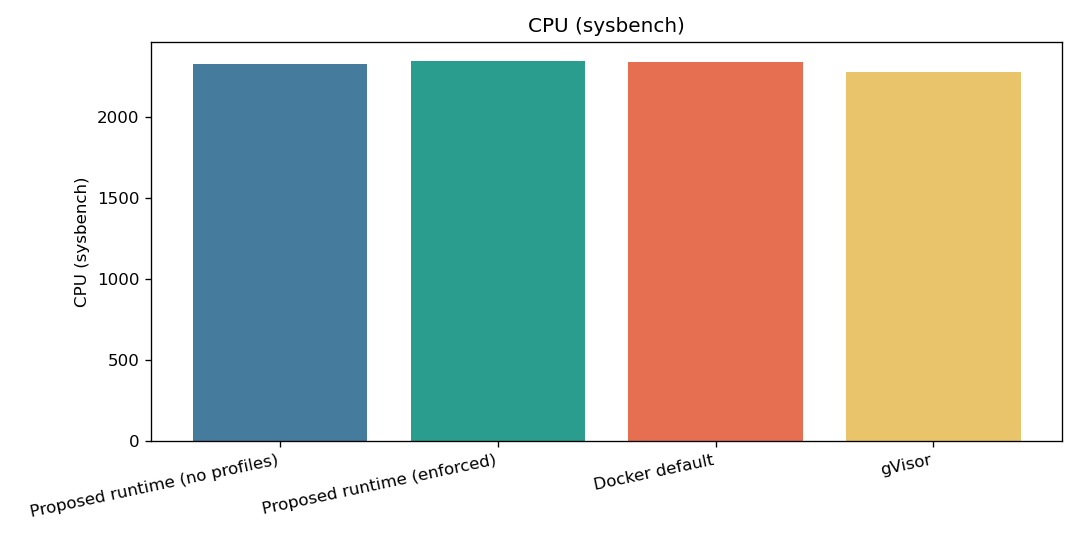
\includegraphics[width=0.48\textwidth]{figs/CPU__sysbench_.png}\hfill
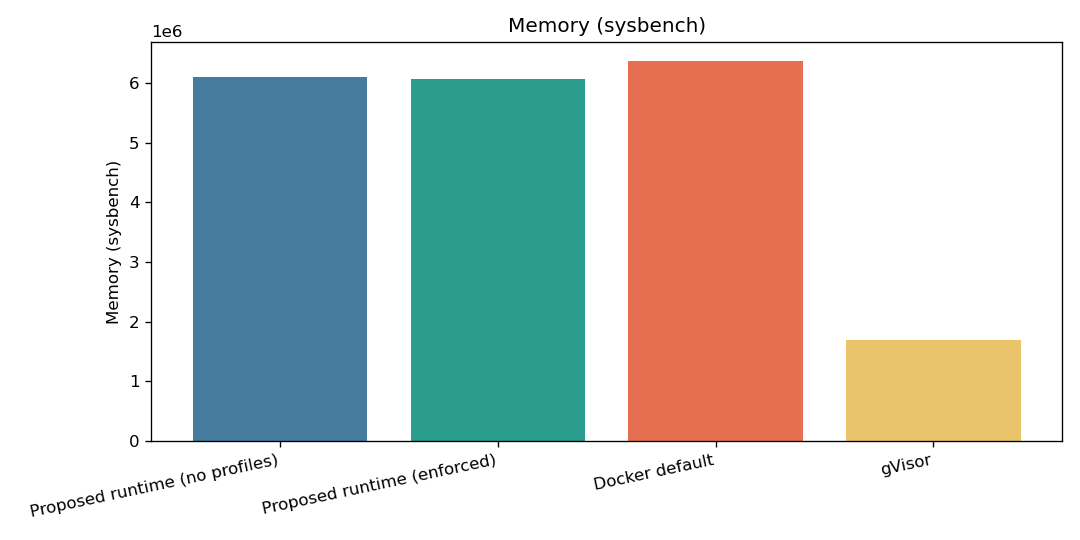
\includegraphics[width=0.48\textwidth]{figs/Memory__sysbench_.png}\\[0.5em]
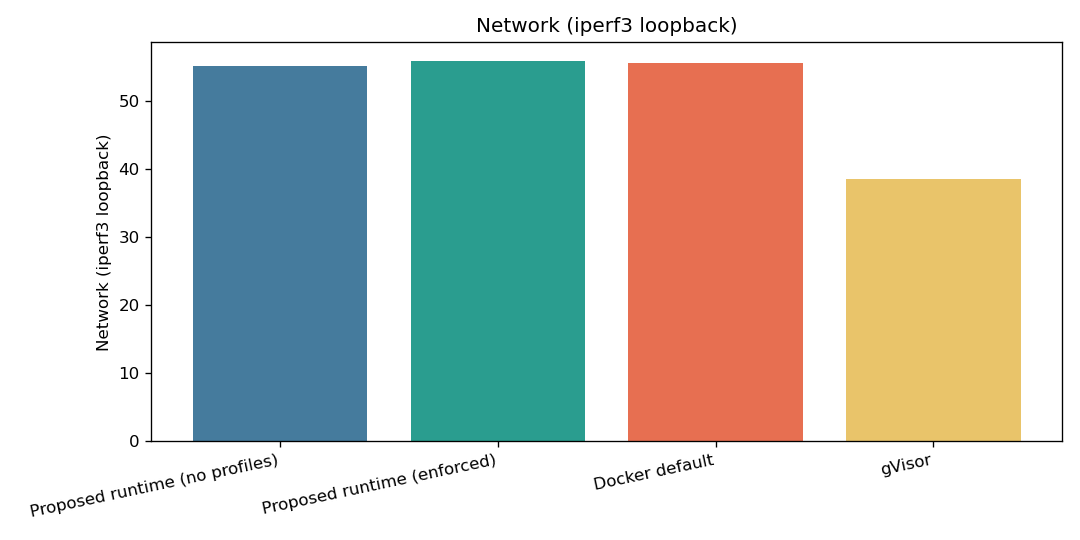
\includegraphics[width=0.48\textwidth]{figs/Network__iperf3_loopback_.png}\hfill
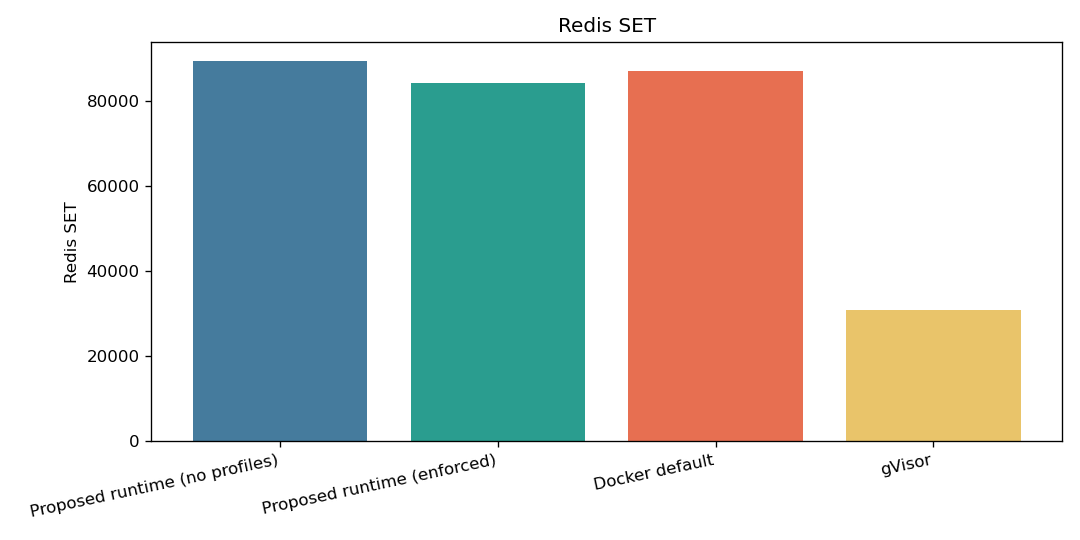
\includegraphics[width=0.48\textwidth]{figs/Redis_SET.png}
\caption{Median throughput by runtime. Left column: enforcement family (\texttt{stock} vs.\ \texttt{proposed}); right panels include Docker and gVisor baselines where applicable.}
\label{fig:enforcement}
\end{figure}

\textbf{Sandbox overhead (gVisor vs.\ Docker).} On the same host, gVisor shows +2.6\% CPU overhead, +73.5\% memory overhead, +30.8\% network overhead, and +65\% Redis overhead relative to Docker-default---confirming that sandboxing trades substantial steady-state throughput for stronger isolation, whereas profile enforcement on a shared-kernel runtime stays near native on compute- and network-bound workloads.

\textbf{Operational notes.} Post-scan AppArmor adjustments for \texttt{/bin/sh}, \texttt{/tmp}, and workload-specific execute paths are applied automatically during profile preparation so functional checks pass; iperf3 additionally requires an unrestricted \texttt{socket} seccomp rule for loopback server/client pairs inside one container namespace. These steps are documented in the harness and are part of the reproducible pipeline, not ad-hoc tuning during measurement.

\subsection{Planned Security Evaluations}\label{sec:eval-security-planned}

The Flask laboratory demonstrates scan-then-enforce against command injection on one realistic workload. The following evaluations are \textbf{not yet reported} and are reserved for a follow-on security campaign beyond \texttt{runc-hardened-test}:

\begin{table}
\caption{Planned security evaluations (placeholders). Each row will report blocked vs.\ allowed outcomes under stock \texttt{runc}, enforced profiles, and selected misconfigurations.}
\label{tab:security-planned}
\centering
\begin{tabular}{p{3.2cm}p{7.8cm}}
\toprule
\textbf{Scenario} & \textbf{Purpose} \\
\midrule
CVE-2019-5736 replay & Test whether enforced profiles limit runc-based container breakout primitives after attacker-controlled writes. \\
Privileged container / \texttt{docker.sock} mount & Measure containment when the deployment grants excessive privileges that profiling cannot fix retroactively. \\
Broad capability or host mount misconfiguration & Quantify defence in depth when operators bypass minimal defaults before scanning. \\
Post-RCE host lateral movement & After simulated compromise inside the namespace, test access to host files, other containers, and cgroup interfaces. \\
Additional vulnerable applications & Generalise RQ2 beyond the Flask monitor to other injection and deserialization patterns. \\
\bottomrule
\end{tabular}
\end{table}

\noindent Until these rows are populated, security claims in this paper are bounded to the laboratory results in Section~\ref{sec:eval-security}.

\section{Analysis}\label{sec:analysis}

\subsection{Security Properties}

The scanner reduces default privileges available at enforcement time. Seccomp removes unused syscalls; capability narrowing removes unused privileged operations; AppArmor adds path-based confinement. Finalisation never unions capability evidence with earlier broad defaults---the output set is rebuilt from an empty set, which keeps results auditable at the cost of scan coverage sensitivity.

The laboratory shows that, for an exercised web workload, automatic profiles block command injection even though the application bug remains in the image. This is a second-line defence analogous to cluster-side recorders, reachable with one CLI flag.

\subsection{Limitations}

\textbf{Dynamic coverage.} Profiles record only behaviour exercised during the scan window. Rare branches, cron jobs, and certificate rotation require representative integration tests.

\textbf{Root workloads.} Capability tracing under-reports checks for UID~0; the runtime warns but does not rewrite the configured user.

\textbf{File capabilities.} Privileges embedded in executable xattrs (e.g.\ \texttt{CAP\_NET\_RAW} on \texttt{ping}) are not yet merged from \texttt{security.capability}; operators must allow-list them explicitly.

\textbf{Measurement environment.} The performance campaign ran inside VirtualBox without KVM or CPU governor pinning; variance is higher than on a dedicated bare-metal or KVM guest. Two launcher families (OCI bundle vs.\ Docker) are required because enforced OCI profiles cannot be applied identically through Docker's runtime path.

\textbf{Incomplete security matrix.} Table~\ref{tab:security-planned} marks escape-class and misconfiguration tests still outstanding.

\subsection{Operational Trade-Off}

gVisor reduces host-kernel exposure more fundamentally than seccomp/AppArmor on a shared kernel~\cite{wang2022,viktorsson2020}. The proposed runtime targets deployments that want \texttt{runc}-class performance and compatibility but cannot operate a cluster-side recorder. Empirical results show enforcement overhead near zero on three of four benchmark workloads and an order of magnitude less than gVisor's sandbox penalty on memory and Redis.

\section{Related Work}\label{sec:related}

Prior runtime comparisons show that default \texttt{runc} is fast but weaker as an isolation boundary, while gVisor trades overhead for stronger isolation~\cite{wang2022,volpert2024,viktorsson2020}. Those studies rarely measure \texttt{runc} with workload-specific enforced profiles. Lopes et al.~\cite{lopes2020} automate seccomp generation; Mattetti and Allouche~\cite{mattetti2020} argue for layered hardening. Cluster-side recorders~\cite{spo2025,inspektorgadget2025} and Tetragon~\cite{tetragon2025} target Kubernetes environments. This work moves the same profiling problem to the OCI runtime layer for developers who can run a container but not a recorder stack.

\section{Conclusion}\label{sec:conclusion}

This paper presented a \texttt{runc} fork that turns workload-specific profile generation into a runtime-side workflow. On the \texttt{runc-hardened-test} laboratory, scan-then-enforce blocked command-injection exploitation while preserving legitimate traffic. On the \texttt{performance-evaluation} harness, enforcing generated profiles on four standard workloads added at most $\approx$5.5\% median throughput overhead relative to the same binary without profiles, while gVisor remained 30--73\% slower than Docker on the same measurements.

Future work will populate Table~\ref{tab:security-planned}, merge file-capability xattrs at scan time, emit Security Profiles Operator-compatible resources, and repeat the performance campaign on a KVM-backed host with cpufreq control. Within the evaluated scope, runtime-side profiling is a practical middle ground between default \texttt{runc} and full sandboxing.

\begin{credits}
\subsubsection{\ackname} Benchmark artefacts and reproducibility scripts are published at \url{https://github.com/dpttk/performance-testing} and \url{https://github.com/dpttk/runc-hardened-test}.

\subsubsection{\discintname} The authors have no competing interests to declare that are relevant to the content of this article.
\end{credits}

\bibliographystyle{splncs04}
\bibliography{ref}

\end{document}
